\documentclass[a4papper,10pt]{article}
\usepackage{etex}
\reserveinserts{28}

\usepackage{xkeyval}[2005/11/25]
\usepackage{eso-pic}
\usepackage{graphicx}
\usepackage{fp}
\usepackage{tikz}
\usetikzlibrary{calc}
\usetikzlibrary{decorations.pathmorphing}
\usetikzlibrary{decorations.pathreplacing} 
\usetikzlibrary{decorations.shapes} 
\usetikzlibrary{shadows}
\usetikzlibrary{arrows}
\usetikzlibrary{shapes,snakes,shapes.geometric,shapes.misc}
\usepackage{multicol}
\usepackage{arabtex}
\usepackage{amsmath,amsfonts,amssymb}
\usepackage{float}
\usepackage{array,booktabs ,tabularx,multirow}
\usepackage{euler}
\usepackage[top=1cm,bottom=0cm,left=1cm,right=1cm]{geometry}
\usepackage{fancyhdr}
\usepackage{xlop}
\usepackage[most]{tcolorbox}
%----------------------------------------...les compteurs..... ----------------------------------------------------------------------%
\newcounter{i}
\setcounter{i}{1}
\newcounter{k}
\setcounter{k}{1}
%----------------------------------------------------------\cadre[x=... ,y=.....,  ]------------------------------------------------------%

% \cadre[			shadow (bool�en),
%					lw = , (�paisseur du trait, en pt)
%					style = , (dashed ou dotted)
%					x = abscisse du sommet en bas � gauche,
%					y = ordonn�e du sommet en bas � gauche,
%					xshadow = d�calage selon x de l'ombre,
%					yshadow = d�calage selon y de l'ombre,
%					color = couleur du cadre,
%					colorshadow = couleur de l'ombre,
%					decoration = nom de la d�coration,
%					doubleline (bool�en) pour pstricks
%				  ]
\makeatletter
\define@cmdkey [PAS] {cadre} {x}{}
\define@cmdkey [PAS] {cadre} {y}{}
\define@cmdkey [PAS] {cadre} {decoration}{}
\define@cmdkey [PAS] {cadre} {shape}{}
\define@cmdkey [PAS] {cadre} {lw}{}
\define@cmdkey [PAS] {cadre} {xshadow}{}
\define@cmdkey [PAS] {cadre} {yshadow}{}
\define@cmdkey [PAS] {cadre} {bordercolor}{}
\define@cmdkey [PAS] {cadre} {incolor}{}
\define@cmdkey [PAS] {cadre} {shadowcolor}{}
\define@cmdkey [PAS] {cadre} {style}{}
\define@boolkey[PAS] {cadre} {shadow}[true]{}
\define@boolkey[PAS] {cadre} {doubleline}[true]{}

\presetkeys    [PAS] {cadre} {	shadow = false,
								lw = 2,
								x = 0.2,
								y = 0.2,
								xshadow =- 0.35,
								yshadow =0.2,
								bordercolor = black,
								incolor = white,
								shadowcolor = gray,
								style = ,
								doubleline = false,
								decoration = , 
								shape = }{}

\newcommand*{\cadre}[1][]{\pasCadre[#1]}

\def\pasCadre[#1]{
	\setkeys[PAS]{cadre}{#1}
	
	\AddToShipoutPicture
	{
		\put(\LenToUnit{\cmdPAS@cadre@x cm},\LenToUnit{\cmdPAS@cadre@y cm})
		{
				\ifPAS@cadre@doubleline
					\edef\dl{double}
				\else
					\edef\dl{}
				\fi
				\begin{tikzpicture}[decoration={\cmdPAS@cadre@decoration,shape=\cmdPAS@cadre@shape}]
					\pgfsetlinewidth{\cmdPAS@cadre@lw pt}
					\ifPAS@cadre@shadow
						\filldraw[
						decorate,
						fill=\cmdPAS@cadre@incolor,
						draw=\cmdPAS@cadre@bordercolor,
						style=\cmdPAS@cadre@style,
						drop shadow={fill=\cmdPAS@cadre@shadowcolor,shadow xshift=\cmdPAS@cadre@xshadow cm,shadow yshift=-\cmdPAS@cadre@yshadow cm},
						\dl] (0,0) -- (0,\paperheight-2*\cmdPAS@cadre@y cm) -- (\paperwidth-2*\cmdPAS@cadre@x cm,\paperheight-2*\cmdPAS@cadre@y cm) -- (\paperwidth-2*\cmdPAS@cadre@x cm,0) -- cycle;
					\else
						\filldraw[
						decorate,
						fill=\cmdPAS@cadre@incolor,
						draw=\cmdPAS@cadre@bordercolor,
						style=\cmdPAS@cadre@style,
						\dl] (0,0) -- (0,\paperheight-2*\cmdPAS@cadre@y cm) -- (\paperwidth-2*\cmdPAS@cadre@x cm,\paperheight-2*\cmdPAS@cadre@y cm) -- (\paperwidth-2*\cmdPAS@cadre@x cm,0) -- cycle;
					\fi
				\end{tikzpicture}
		}
	}
}

\def\nocadre{\ClearShipoutPicture}
%-----------------------------------------------\entete---------------------------------------------------------------------------%
\newcommand{\entete}{
\noindent
\begin{tabularx}{\textwidth}{|r  ||||X|||| r |}
\toprule
\RL{AlmdT AlzmnyT : sA`tAn}
&
\centering \RL{{\LARGE Al-'imt.hAn Al|m|.hly Al|m|w.hd }}
&
 \RL{_tAnwyT `bd Alkrym Alx.tAby Al-'i`dAdyT}\\
 \RL{AldwrT : $II$}& \centering   \RL{\Large{fy m|AdT AlryA.dyAt}}&\RL{nyAbT tAwryrt} \\
 \RL{Alm`Aml : $3$} & \centering  \RL{AlsnT Al_tAl_tT 'i`dAdy} & \RL{dabdw}\\
 \bottomrule
\end{tabularx}
}
%--\exercice[bareme,bar=...]{........}------------------------------%
\define@cmdkey[EX]{exo}{bar}{}
\define@boolkey[EX]{exo}{bareme}[true]{}
\presetkeys[EX]{exo}{bar= ,bareme=false}{}
\newcommand{\exercice}[2][]{
\setkeys[EX]{exo}{#1}
\setcounter{k}{1}
\tikzstyle{mybox} = [ draw, very thick,rounded corners=3mm, inner sep=10pt, inner ysep=10pt]
\tikzstyle{fancytitle} =[fill=white, text=black,inner ysep=0pt,inner xsep=2pt]
\noindent
\begin{tikzpicture}
\node [mybox] (box){%
    \begin{minipage}{0.88\linewidth}
        #2 
    \end{minipage}
};
\node[fancytitle, left=10pt] at (box.north east) {{\large \arabic{i}\RL{Altmryn}}};
\ifEX@exo@bareme
\node[fancytitle] at (box.north){\RL{nq.t} \cmdEX@exo@bar };
\fi
\end{tikzpicture}%
\stepcounter{i}
}
%-----------\question[bareme,bar=...]{......}----------------------%
\define@cmdkey[EX]{qst}{bar}{}
\define@boolkey[EX]{qst}{bareme}[true]{}
\presetkeys[EX]{qst}{bar= ,bareme=false}{}
\newcommand{\question}[2][]{
\setkeys[EX]{qst}{#1}
\ifEX@qst@bareme
	\ifdim \cmdEX@qst@bar pt  < 2 pt
\begin{arabtext}
$-\arabic{k}$ \marginpar{ \cmdEX@qst@bar{} pt} #2
\end{arabtext}
	\else
\begin{arabtext}
$-\arabic{k}$ \marginpar{ \cmdEX@qst@bar{} pts} #2
\end{arabtext}
	\fi
\else
\begin{arabtext}
$-\arabic{k}$ #2
\end{arabtext}
\fi
\stepcounter{k}
}
%----------\devoir[niv=... , num=..., date=..., ds=...]----------%
\define@boolkey[EX]{devoir}{ds}[true]{}
\define@cmdkey[EX]{devoir}{niv}{}
\define@cmdkey[EX]{devoir}{num}{}
\define@cmdkey[EX]{devoir}{date}{}
\presetkeys[EX]{devoir}{niv=$3$,num=$1$,ds=true,date=}{}
\newcommand{\devoir}[1][]{
\setkeys[EX]{devoir}{#1}

\begin{tikzpicture}
\node [draw,shape=chamfered rectangle] (box1){%
    \begin{minipage}{0.2\textwidth}
      \center \cmdEX@devoir@date \RL{AltAryx :{} }
    \end{minipage}
};
\end{tikzpicture}%
\ifEX@devoir@ds
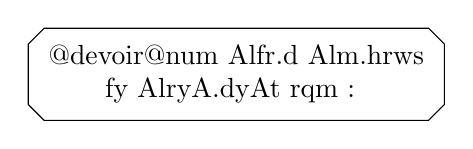
\begin{tikzpicture}
\node [draw,shape=chamfered rectangle] (box2){%
    \begin{minipage}{0.4\textwidth}
       \center\cmdEX@devoir@num \RL{Alfr.d Alm.hrws fy AlryA.dyAt rqm :{} }
    \end{minipage}
};
\end{tikzpicture}%
\else
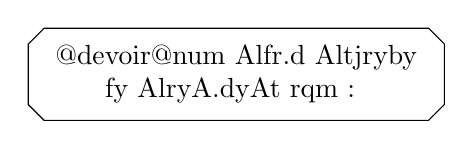
\begin{tikzpicture}
\node [draw,shape=chamfered rectangle] (box2){%
    \begin{minipage}{0.4\textwidth}
       \center\cmdEX@devoir@num \RL{Alfr.d Altjryby fy AlryA.dyAt rqm :{} }
    \end{minipage}
};
\end{tikzpicture}%
\fi
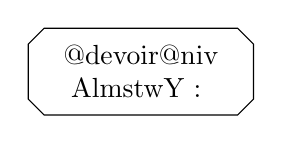
\begin{tikzpicture}
\node [draw,shape=chamfered rectangle] (box3){%
    \begin{minipage}{0.2\textwidth}
 \center\cmdEX@devoir@niv \RL{AlmstwY :{} }     
    \end{minipage}
};
\end{tikzpicture}%
}
%------------------------------------------------\serie[titre=..]-----------------------------------------------------------------------------%

\define@cmdkey[EX]{serie}{titre}{}
\presetkeys[EX]{serie}{titre=\RL{`nwAn Aldrs}}{}
\newcommand{\serie}[1][]{
\setkeys[EX]{serie}{#1}
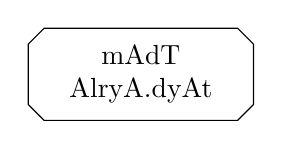
\begin{tikzpicture}
\node [draw,shape=chamfered rectangle] (box1){%
    \begin{minipage}{0.20\textwidth}
       \center\RL{mAdT AlryA.dyAt}
    \end{minipage}
};
\end{tikzpicture}%
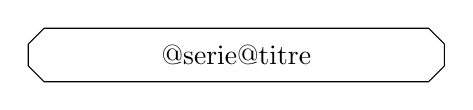
\begin{tikzpicture}
\node [draw,shape=chamfered rectangle] (box2){%
    \begin{minipage}{0.40\textwidth}
      \center\cmdEX@serie@titre
    \end{minipage}
};
\end{tikzpicture}%
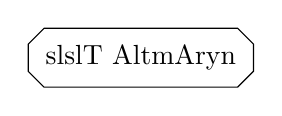
\begin{tikzpicture}
\node [draw,shape=chamfered rectangle] (box3){%
    \begin{minipage}{0.20\textwidth}
   \center\RL{slslT AltmAryn}
    \end{minipage}
};
\end{tikzpicture}%
}
\makeatother

\begin{document}
\devoir[num=5,niv=1,ds=\RL{Alm.hrws},date=18/04/2018]

\exercice[bareme,bar=6]{
\begin{minipage}{0.6\linewidth}
\definecolor{qqwuqq}{rgb}{0,0.39,0}
\definecolor{xdxdff}{rgb}{0.49,0.49,1}
\definecolor{qqqqff}{rgb}{0,0,1}
\definecolor{cqcqcq}{rgb}{0.75,0.75,0.75}
\begin{tikzpicture}[line cap=round,line join=round,>=triangle 45,x=1.0cm,y=1.0cm,rounded corners=0pt]
\clip(-3.63,0.5) rectangle (4.17,5.88);
\draw [shift={(1,2)},color=qqwuqq,fill=qqwuqq,fill opacity=0.1] (0,0) -- (143.13:0.55) arc (143.13:180:0.55) -- cycle;
\draw [shift={(1,2)},color=qqwuqq,fill=qqwuqq,fill opacity=0.1] (0,0) -- (180:0.55) arc (180:251.57:0.55) -- cycle;
\draw [domain=-3.63:4.17] plot(\x,{(--25-0*\x)/5});
\draw [domain=-3.63:4.17] plot(\x,{(--10-0*\x)/5});
\draw [domain=-3.63:4.17] plot(\x,{(--1-3*\x)/-1});
\draw [domain=-3.63:4.17] plot(\x,{(-11--3*\x)/-4});
\draw [shift={(1,2)},color=qqwuqq] (143.13:0.55) arc (143.13:180:0.55);
\draw [shift={(1,2)},color=qqwuqq] (143.13:0.45) arc (143.13:180:0.45);
\draw [shift={(1,2)},color=qqwuqq] (180:0.55) arc (180:251.57:0.55);
\draw[color=qqwuqq] (0.6,1.71) -- (0.51,1.65);
\begin{scriptsize}
\fill [color=qqqqff] (1,2) circle (1.5pt);
\draw[color=qqqqff] (1.33,2.28) node {$A$};
\fill [color=qqqqff] (2,5) circle (1.5pt);
\draw[color=qqqqff] (2.32,5.27) node {$B$};
\draw (3.9,5.27) node {$(D)$};
\draw (3.32,2.27) node {$(D')$};
\fill [color=qqqqff] (-3,5) circle (1.5pt);
\draw[color=qqqqff] (-2.88,5.41) node {$C$};
\fill [color=xdxdff] (-2,2) circle (1.5pt);
\draw[color=xdxdff] (-1.85,2.25) node {$D$};
\fill [color=xdxdff] (0.66,0.97) circle (1.5pt);
\draw[color=xdxdff] (0.79,0.57) node {$E$};
\draw[color=black] (0.06,2.36) node {$50^{\circ}$};
\draw[color=black] (0.19,1.54) node {$60^{\circ}$};
\end{scriptsize}
\end{tikzpicture}
\end{minipage}
\begin{minipage}{0.3\linewidth}
on considere la figure ci contre ,
 $(D) // (D')$  .

Donner la mesure des angles de triangle  $ABC$ .
$$\widehat{ABC}=.............. $$
$$\widehat{ACB}=..............  $$
$$\widehat{BAC} =.............. $$

\end{minipage}
}

\exercice[bareme,bar=6]{
citez les proprietes carateristiques du parallelogramme ?

1- tracer un parallelogramme ABCD de centre O .

2- trace E le symetrique de A par rapport a D .

3- trace F le symetrique de C par rapport a B .

4- montrer que AFBD est un parallelogramme .
%\question{byn anna $BCED$ mtwAzy Al-'a.dlA`}
%\question{byn anna $O$ mnt.sf $[EF]$}
}

\exercice[bareme,bar=5]{
\begin{itemize}
\item $ABCD$ parallelogramme tel que  $\widehat{ABC}=90^{\circ}$ donc il est  .............................................
\item $ABCD$ parallelogramme tel que  $AB=AD$ donc il est .............................................
\item $ABCD$ parallelogramme tel que $(AC)\perp (BD)$ donc il est .............................................
\item $ABCD$ parallelogramme tel que $AC=BD$ donc il est .............................................
\item $ABCD$ parallelogramme tel que $AC=BD$  w $(AC)\perp (BD)$ donc il est .............................................
\end{itemize}
}

\exercice[bareme,bar=3]{
\begin{minipage}{0.4\linewidth}
\definecolor{uuuuuu}{rgb}{0.27,0.27,0.27}
\definecolor{qqqqff}{rgb}{0,0,1}
\begin{tikzpicture}[line cap=round,line join=round,>=triangle 45,x=1.0cm,y=1.0cm,scale=0.75]
\clip(-4.7,-0.38) rectangle (2.86,6.52);
\draw(-1,3) circle (1.52cm);
\draw(-1,3) circle (3cm);
\draw [domain=-4.7:2.86] plot(\x,{(-3.88-1.24*\x)/-0.88});
\draw [domain=-4.7:2.86] plot(\x,{(--9-0*\x)/3});
\draw [dash pattern=on 1pt off 2pt on 4pt off 4pt] (-0.12,4.24)-- (0.52,3);
\draw [dash pattern=on 1pt off 2pt on 4pt off 4pt] (0.52,3)-- (-1.88,1.76);
\draw [dash pattern=on 1pt off 2pt on 4pt off 4pt] (-1.88,1.76)-- (-2.52,3);
\draw [dash pattern=on 1pt off 2pt on 4pt off 4pt] (-2.52,3)-- (-0.12,4.24);
\draw (2,3)-- (-0.12,4.24);
\draw (-0.12,4.24)-- (-4,3);
\draw (-4,3)-- (-1.88,1.76);
\draw (-1.88,1.76)-- (2,3);
\begin{scriptsize}
\fill [color=qqqqff] (-1,3) circle (1.5pt);
\draw[color=qqqqff] (-0.76,2.88) node {$O$};
\fill [color=qqqqff] (-0.12,4.24) circle (1.5pt);
\draw[color=qqqqff] (0.32,4.38) node {$B$};
\fill [color=qqqqff] (2,3) circle (1.5pt);
\draw[color=qqqqff] (2.16,3.28) node {$C$};
\fill [color=uuuuuu] (-4,3) circle (1.5pt);
\draw[color=uuuuuu] (-4.14,2.54) node {$A$};
\fill [color=uuuuuu] (-1.88,1.76) circle (1.5pt);
\draw[color=uuuuuu] (-1.84,1.3) node {$D$};
\fill [color=uuuuuu] (-2.52,3) circle (1.5pt);
\draw[color=uuuuuu] (-2.8,2.82) node {$E$};
\fill [color=uuuuuu] (0.52,3) circle (1.5pt);
\draw[color=uuuuuu] (0.76,3.32) node {$F$};
\end{scriptsize}
\end{tikzpicture}
\end{minipage}
\begin{minipage}{0.6\linewidth}

On considere la figure tel que $(C)$ et $(C')$ deux cercles ayant le meme centre $O$

1- quel est la nature de $EBFD$ ? justifier votre reponce
....................................................................
..................................................................

2- montrer que  $ABCD$  est un parallelogramme ? 
....................................................................
..................................................................

3- Si  $(AC)\perp (BD)$ , determiner la nature de  $EBFD$ et $ABCD$ 
....................................................................
..................................................................
\end{minipage}
}










\end{document}